\documentclass{article}
\usepackage{enumerate}
\usepackage{tikz}
\usepackage{float}
\usepackage[bottom]{footmisc}
\usepackage{hyperref}
\usepackage{amsfonts}
\usepackage{graphicx}

\usetikzlibrary{graphs} 
\usetikzlibrary{graphdrawing}
\usetikzlibrary{graphs.standard}
\usetikzlibrary{positioning}
\usegdlibrary{layered,circular,force}
\title{Hamiltonian Cycles in Square Lattice Subgraphs}
\begin{document}
\date{\vspace{-5ex}}
\maketitle

\section{Abstract}
This paper identifies a certain visual property of boundaries of right-angled walls, found in the video game Pacman, where corners are rounded and walls are straight and clamped in alignment with the normal of the path which they face. The walls form a closed boundary. The 2-dimensional gridded nature of wall placement allows them to be represented using a square lattice graph. With the aim of finding the direction towards which they are clamped, so as to recreate the visual properties of the walls in Pacman, we devise a polynomial-complexity algorithm for finding a hamiltonian cycle in square-lattice subgraphs, and establish the criteria for its devisability.

\section{Problem Introduction}
Pacman is a video game which utilizes textures of 8x8 pixels to render its core components as can be seen in Figure 1. 

\begin{figure}[H]
\centering
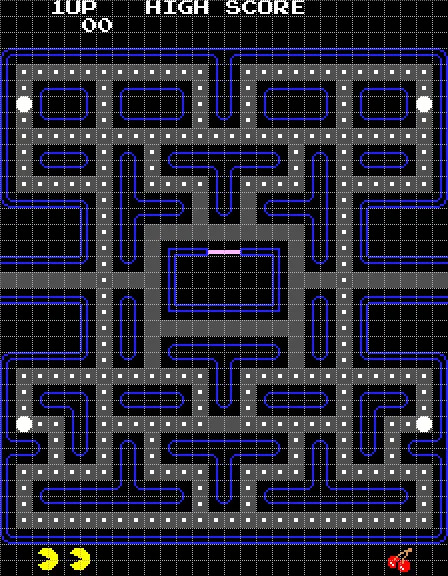
\includegraphics[width=0.4\linewidth]{Image-1.jpg}
\caption [Pacman level divided into squares of 8x8 pixels.]{Pittman, Jamey. Tiles. 2023, Gamedeveloper.com.}
\label{Pacman Level Grid}
\end{figure}

Since the pixel length of a wall is 1 pixel, the wall textures all contain an asymmetry as seen in Figure 2 and 3.

\begin{figure}[H]
\centering

\includegraphics[width=0.5\linewidth]{Image-2.png}\hfill
\caption {A single wall square texture.}
\label{Straight wall texture}
\end{figure}

\begin{figure}[H]
\centering

\includegraphics[width=0.5\linewidth]{Image-3.png}\hfill
\caption {Square texture of corner.}\label{fig:CornerTexture}
\end{figure}

Because of this asymmetry, it must be decided in what direction walls are clamped to ensure visual consistency. When all walls are clamped in the same direction we receive unsatisfactory results as seen in Figure ~\ref{Wall Texture Asymmetry}.

\begin{figure}[H]
\centering
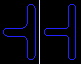
\includegraphics[width=0.5\linewidth]{Image-4.png}
\caption {Left - Incorrect orientation of tiles. Right - Correct orientation with walls clamped to appropriate direction.}\label{Wall Texture Asymmetry}
\end{figure}

This problem will be reduced to the basic elements of graph theory.

\section{Definitions}

\begin{enumerate}[I.]
\item We define a graph as a set $G=\lbrace V,E \rbrace$. $V$ is a set of vertices. $E$ is a set of edges. Vertices can be thought of as standalone points. Edges are connections between vertices, where an edge $e\in E, $ for $ V_{x},V_{y}\in V, e=\lbrace V_{x},V_{y} \rbrace $, connects vertices $V_{x}$ and $V_{y}$.  A graph can be represented by a drawing. For the example graph $G=\lbrace E,V \rbrace$, where $E=\lbrace a,b,c,d \rbrace $ and $ V=\{\{a,b\},\{b,c\},\{c,d\},\{d,a\}\}$ we can draw the following diagram.

\begin{figure}[H]
	\centering
	\tikz [every node/.style={draw,circle}]
		\graph [simple necklace layout, node distance=2cm] {
			a--b--c--d--a
	};
	\caption{A graph of four vertices that are all bidirectionally connected to each other.}
\end{figure}

Here are several other examples of graphs (these are not essential to the paper, but can give a broader idea of what a graph can be):

\begin{figure}[H]
	\centering
	\tikz [every node/.style={draw,circle}] \graph {a--b--c--d};
	\caption{A "spine" graph.}
\end{figure}

\begin{figure}[H]
	\centering
	\tikz [every node/.style={draw,circle}] \graph { subgraph K_n [n=6, clockwise] };
	\caption { A complete graph. }
\end{figure}

\begin{figure}[H]
	\centering
	\tikz [every node/.style={draw,circle}] \graph { a -> {b, c} -> d };
	\caption {A directed graph. Each edge is assigned a direction indicated by the arrows.}
\end{figure}

\item A \textit{\textbf{walk}} for a graph $G=\{V,E\}$ is an alternating sequence of vertices in $V$ and edges in $E$.\footnote{P. Bogart, Kenneth. Introductory Combinatorics. San Diego CA, Academic Press, 2000. p. 204.} It has the form ${v_1}{e_1}{v_2}{e_2}{v_3}{e_3}...{e_{n-1}}{v_n}$, where $e_k\in E,v_l\in V, 1\leq k\leq n-1, 1\leq l\leq n$. A walk in which only the first and last vertices are equal, is called a \textit{\textbf{cycle}}.\footnote{P. Bogart. p. 204} The following diagrams are examples of walks:

\begin{figure}[H]
	\centering
	\tikz [every node/.style={draw,circle}] \graph [simple, grow right=2cm] {
		 subgraph K_n [n=6, clockwise];
 		 {[edges={red,thick}] 1 ->  2 -> 5 -> 3 -> 4 -> 6}
	};
	\caption {A path with vertices 1,2,5,3,4,6, and the respective edges to join them}
\end{figure}

\begin{figure}[H]
	\centering
	\tikz [every node/.style={draw,circle}] \graph [grid placement] { 
		subgraph Grid_n [n=9];

		{[edges={red,thick}] 1 -> 2 -> 3 -> 6 -> 5 -> 8 -> 7 -> 4 -> 1}
	};
	\caption {A path with vertices 1,2,3,6,5,8,7,4,1. The walk comes back to the first vertex through a string of unique vertices and is thus a cycle.}
\end{figure}

\item A \textit{\textbf{Hamiltonian cycle}} for a graph $G=\{V,E\}$ is a cycle containing every vertex $v\in V$.\footnote{P. Bogart. p. 210} Since it is a cycle, it comes back to the first vertex of the walk, but, by definition, does not walk onto the any other vertex on more than one occasion. The following is an example of a hamiltonian cycle:

\begin{figure}[H]
	\centering
	\tikz [every node/.style={draw,circle}] \graph [grid placement] { 
		subgraph Grid_n [n=36];
		{[edges={red,line width=2pt}] 1 -> 2 -> 3 -> 9 -> 15 -> 16 -> 10 -> 4 -> 5 -> 6 -> 12 -> 11 -> 17 -> 18 -> 24 -> 23 -> 29 -> 30 -> 36 -> 35 -> 34 -> 28 -> 22 -> 21 -> 27 -> 33 -> 32 -> 31 -> 25 -> 26 -> 20 -> 19 -> 13 -> 14 -> 8 -> 7 -> 1}
	};
	\caption {A Hamiltonian cycle. Although it does not include every edge, it includes each vertex exactly once, before arriving at the starting vertex (Note that the starting vertex is abritrary as it is a loop; any vertex can be considered the starting vertex).}
\end{figure}

\item A square lattice graph $G=\{V,E\}$ is a graph in which each vertex can be distinctly mapped onto an integer tuple $(x,y)$, where $x,y\in \mathbb{Z}$, and where the edges of a vertex $v\in V$ only connect to the respective vertices of a distance of 1 in each cardinal direction. Essentially, a square lattice graph is a graph created out of some points on a coordinate grid, that for a coordinate $(x,y)$ are only ever connected by edges to coordinates with coordinate points $(x+1,y), (x-1,y), (x,y+1)$, or $(x,y-1)$. Figure  5, 6, 8, 10 and 11 are all examples of square lattice graphs.

\end{enumerate}

\section{First Approach}
\end{document}